\documentclass[letterpaper,11pt]{article}
\usepackage{array}
\usepackage{graphicx}
\usepackage{subcaption}
\usepackage{pdfpages}
\usepackage{changepage}
\usepackage{color}
\usepackage[hyphens,spaces,obeyspaces]{url}
\usepackage[colorlinks=true,urlcolor=blue,citecolor=black]{hyperref}
\usepackage[title]{appendix}
\usepackage{float}
\usepackage{listings}
\usepackage{amsmath}
\usepackage{cleveref}
\usepackage{tikz}
\usepackage{arydshln}
\usetikzlibrary{shapes,arrows}
\usetikzlibrary{positioning}
\usepackage[margin=1.5in]{geometry}
\linespread{1.1}
\setlength{\parindent}{30pt}
\setlength{\emergencystretch}{3em}
\setlength\dashlinedash{0.2pt}
\setlength\dashlinegap{1.5pt}
\tikzstyle{arrow} = [thick,->,>=stealth]
\tikzstyle{utxo} = [
    rectangle, minimum width=3.8cm, minimum height=4cm, text centered, text width=3.8cm,
    scale=0.85, draw=black, font=\ttfamily]
\tikzstyle{contract} = [
    rectangle, minimum width=3.8cm, minimum height=4cm, text centered, text width=3.8cm,
    scale=0.85, draw=black, font=\ttfamily, fill=gray!5]

\title{\LARGE BAND\\
    \Large Unleashing Tokenized Economy}
\author{
        Soravis Srinawakoon\\
        \small\href{mailto:soravis@bandprotocol.com}
            {\nolinkurl{soravis@bandprotocol.com}}
    \and
        Sorawit Suriyakarn\\
        \small\href{mailto:swit@bandprotocol.com}
            {\nolinkurl{swit@bandprotocol.com}}
    }
\date{\today\\\small Draft Version 0.1.1}
\begin{document}

\maketitle

\begin{abstract}

Band Protocol is a decentralized, permissionless blockchain protocol to create tokenized marketplace and token-curated community. Band Protocol enables seamless issuance of personalized Community Token through a continuous bonding curve, a smart contract that mints and burned personalized token through a predefined mathematical function based on current circulating supply. Any entities ranging from businesses, brands and celebrities can create a loyal token-curated community with personalized tokens. Personalized Community Token is a utility token representing primary currency, subscription, discount, reward point, or any other use cases within the community as defined by the Community Manager.

Band Protocol standardizes Product Token as a way for community manager to issue products and services. It enables both tokenized real-world products as well as new digital asset creation such as rare digital collectibles and attention token.

Band Protocol enables the creation of subscription business model. Followers can stake their Community Token to a staking contract and receive regular benefits similar to normal subscription or membership. Band Protocol allows Community Manager to define their subscription tier and discount token. Discount token is a tokenized discount voucher used to reward loyal followers and incentivize active participants rather than speculators. The amount of discounts can be customized by Community Manager and in general is proportionate to the amount of total network value. Discount tokens will be an incentive for loyal followers to stake their tokens and promote the growth of the community.

Band Token is the native utility token on the delegated-proof-of-stake Band Chain. Band Token are used to secure the network, provide global liquidity to every Community Token, and act as a governance token for future protocol upgrade.

\end{abstract}

\newpage
{
\hypersetup{linkcolor=black}
\tableofcontents
}
\newpage

\section{Introduction}

\subsection{Tokenized Economy}

A typical market-based economy involves the exchange of goods and services through barter or a medium of exchange. Traditionally, buyers exchange physical coins and banknote with physical products or services offered by sellers. As technology progresses, Internet has enabled digital economy whereby goods and services are being exchanged with digital money. E-commerce experiences exponential growth as people can conveniently conduct transaction with people across the world. Centralized companies start to dominate marketplace platform and payment gateway which are key enablers of the digital economy.

Blockchain and crypto assets are giving rise to yet another revolution in the economy. Bitcoin~\cite{nakamoto}, the first cryptocurrency, becomes the first decentralized currency which enables trustless, censorship-resistant payment. Cryptocurrency such as Bitcoin allows anyone to send transaction to anyone around the world at a fraction of a cost and a fraction of time required for traditional financial institutions to conduct similar transaction. As payment and currency are being tokenized, traditional asset is slower to experience similar tokenization process. Regulation and usability are two key factors that hinder the explosive growth of asset tokenization. Asset tokenization has clear benefits:
\begin{itemize}
\item Global accessibility
\item Liquidity premium
\item Low transaction fee
\item Transparency
\item Security
\end{itemize}

Similar to how physical trade transitions to digital trade by the advancement of the Internet, the next era of commerce is the transition from centralized digital trade to decentralized token trade. Tokenized economy will become prevalent as both real-world assets and payment are being tokenized. Band Protocol enables asset tokenization and creates a standard platform for tokenized economy.
\newpage

\subsection{Token-curated Community}
Typically, economy centers around community with common shared interest. There are multiple layers of community depending on the focus. A country is one big community where everyone shares geographical border, culture, tradition, customs and beliefs. Soccer players and followers together is another community where everyone shares interest in the sport which leads to an economic activity around soccer team and players. This leads to two sides of participant in the community: buyers and sellers. While they share similar interest in the same community, they often have conflicting needs as both sides try to maximize their own utility at the expense of the other side. Soccer team would raise their ticket price as they gain more popularity while their loyal followers have to keep paying more. Conversely, followers will not go out of their way to promote their favorite artist because they have very little economic incentive to do so. Their incentives are not truly aligned.

Crypto asset becomes the answer to which community members can finally have an aligned incentive to grow the community together. A token-curated community is a community centered around a personalized Community Token whose value closely tie to the overall network value of the community. Community Token acts as a shared economic incentive for both buyers and sellers to promote the growth of the community. Band Protocol standardizes the creation of token-curated community and details how personalized Community Token's value can be derived from overall community value through staking and discount mechanism.

%Currently companies, brands and celebrities struggle to engage with their loyal customers and followers. They mostly utilize social media channels such as Facebook, Twitter, and Instagram to cultivate their community. However, it is becoming more difficult to monetize their fan base. Many celebrities try to monetize their followers by advertising products from other companies to their followers, which is not always in the best interest of the community. For example, recent Thai celebrities are facing lawsuit because they advertise non-FDA-approved cosmetics. Influencers accept payment to promote products inorganically which misleads their followers. Similarly, content distributor channel like Youtube and Spotify are taking a big cut from content provider. Newcomers find themselves much more difficult to compete for attention and create network effect, which was originally promised by these platforms.


\subsection{Use Cases}
\begin{itemize}
\item A new musician creates a new community and publishes her first album. She cultivates and rewards early adopters through her Community Token. By having skin-in-the-game token, early adopters rally behind her success and help her grow the community.
\item Bruno Mars issue Bruno Token which can be staked to receive constant discount for all future products, priority queue to purchase concert ticket, and right to access VIP zone during meet and greet session. Bruno Mars also sell rare digital cards which contain non-public photos of the band and digital artwork.
\item Established company creates a community to curate information around a company and reward active participants with community token. Similar to how Barilla encourages followers to post new recipe on Facebook Page, now active participants can receive Barilla Token to purchase Barilla products as an incentive to curate information inside Barilla community.
\end{itemize}

\subsection{BAND Architecture} \label{sec:band-architecture}

BAND architecture consists of three main layers shown in figure~\ref{fig:pyramid}:

\begin{itemize}
\item \textbf{BAND Blockchain Layer} provides backbone blockchain network to support the entire BAND ecosystem. This includes design of cryptographic algorithm for public-private key management, gas allocation, blockchain internal state representation, on-chain price oracle and native BAND Token.
\item \textbf{BAND Protocol Layer} provides standard contracts to facilitate tokenized economy by enabling creation of personalized-token-curated community, tokenized products, token subscription model, discount token, attention curation market, etc.
\item \textbf{Application Layer} is the consumer-facing application that utilize the underlying BAND blockchain and protocol and serve real-world needs. Any developers can create a solution on top of open, permissionless BAND Protocol. Campbase will be the first application built on top of BAND.
\end{itemize}

\begin{figure}[h]
    \centering
    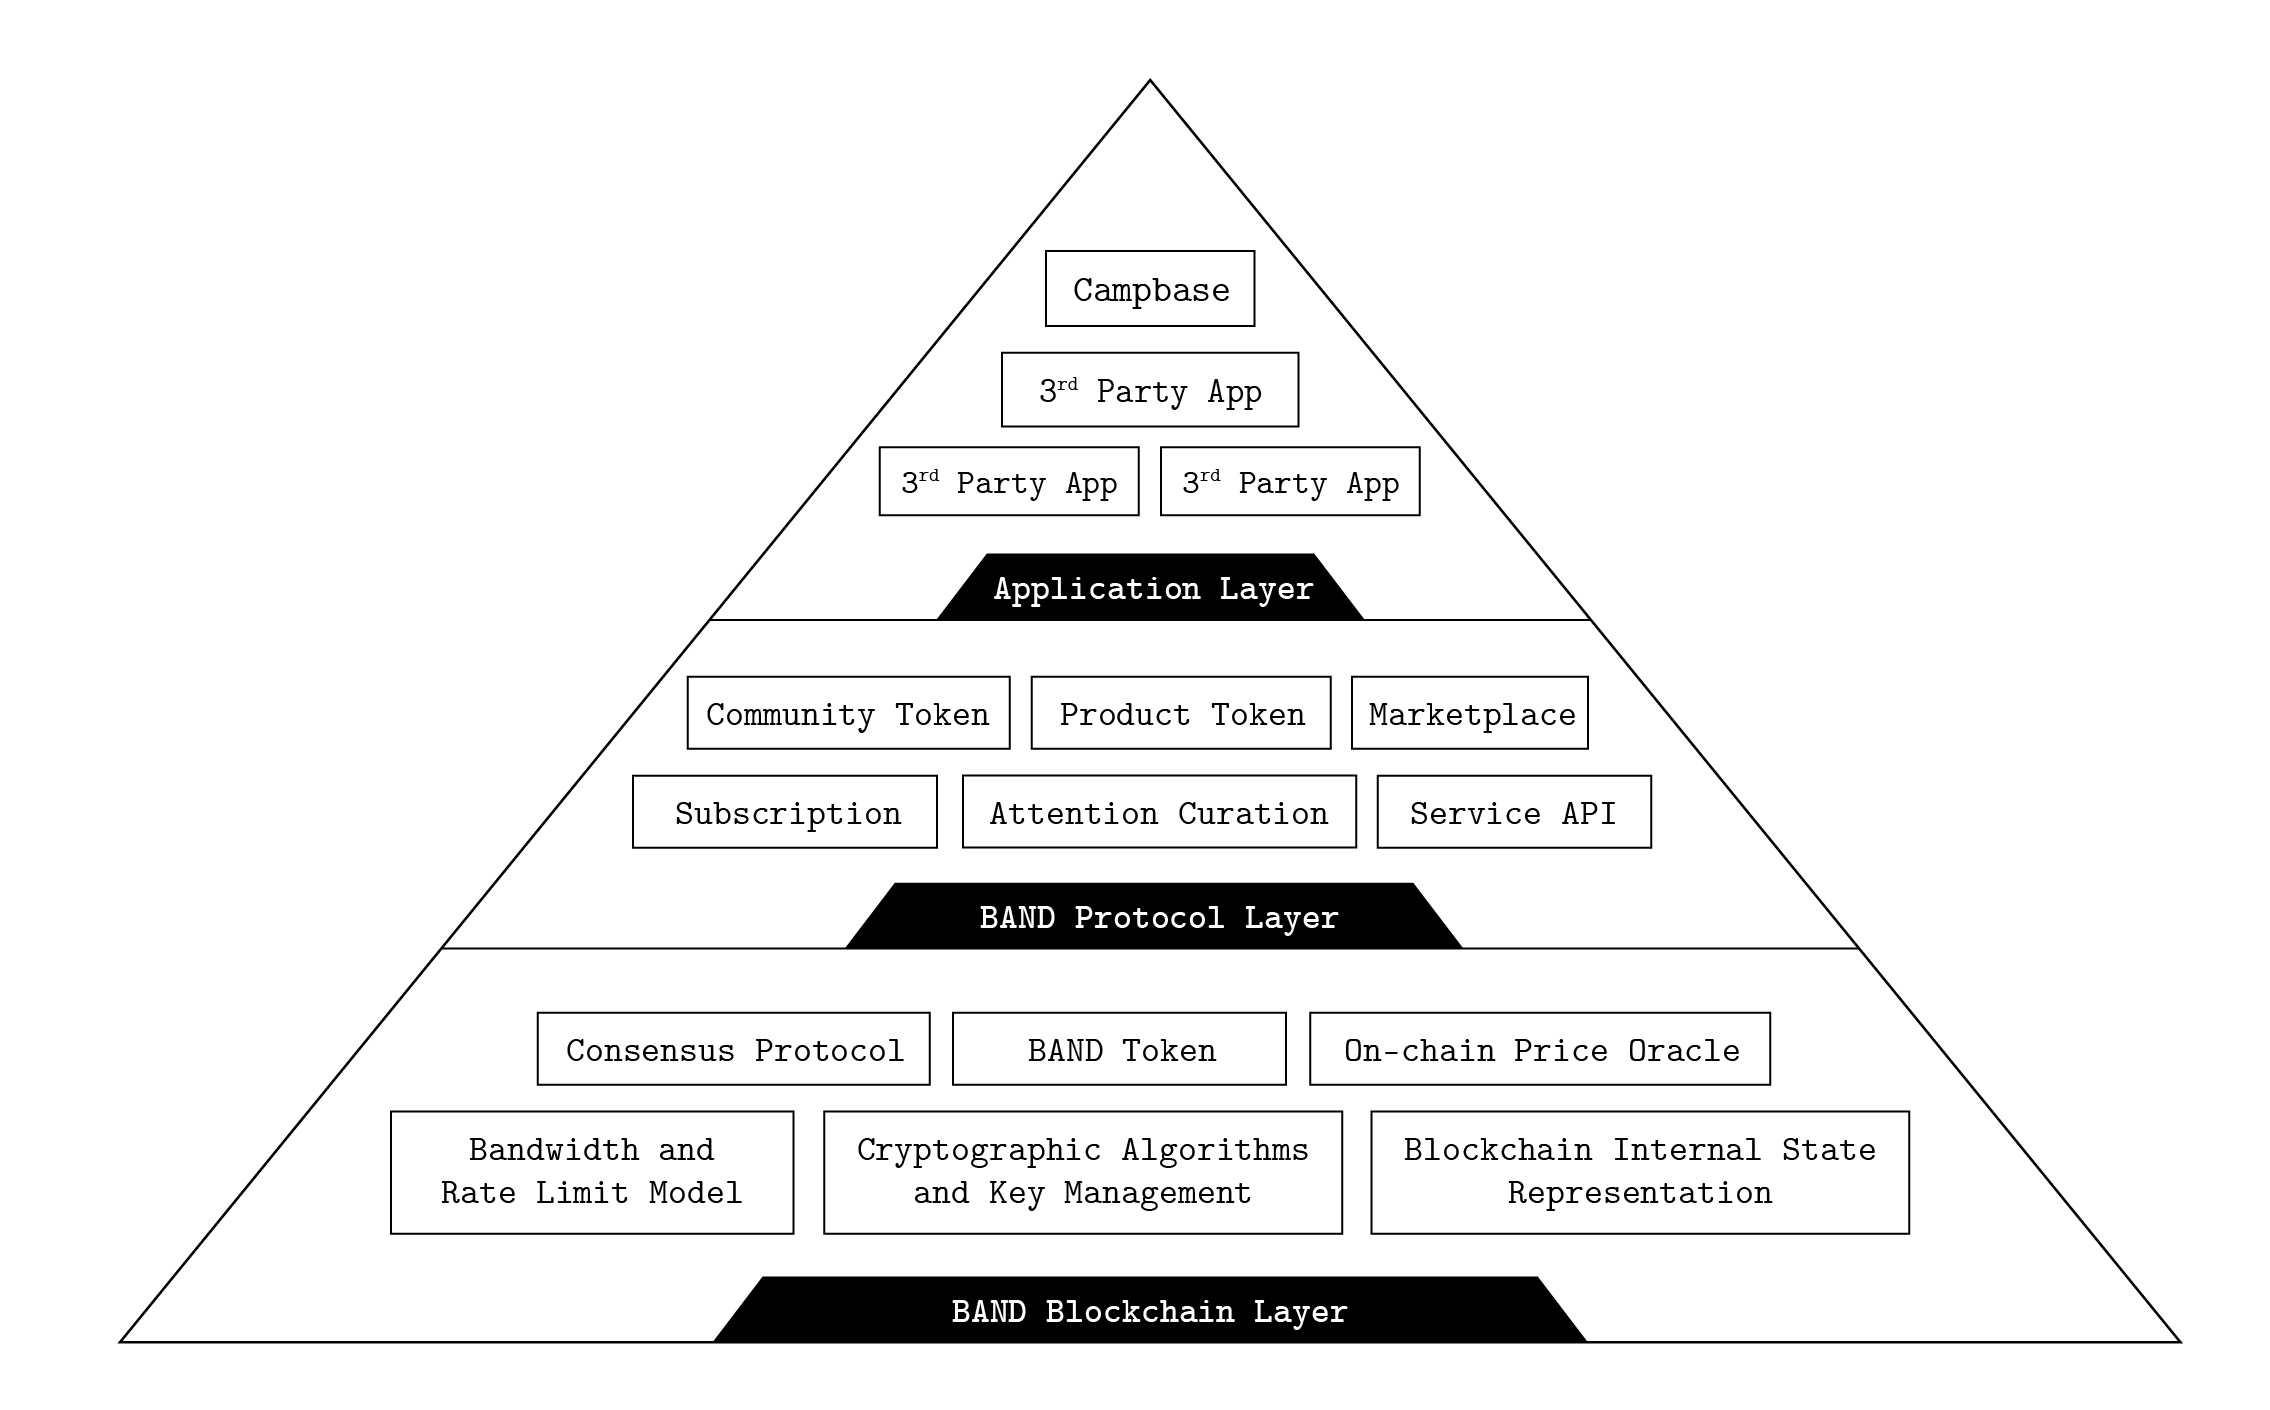
\includegraphics[width=1.05\textwidth]{figures/pyramid}
    \caption{Overview of BAND architecture}
    \label{fig:pyramid}
\end{figure}

\clearpage
\newpage

\section{Blockchain Layer} \label{sec:blockchain-layer}
This section discusses the overview of the blockchain layer in the BAND architecture. Please refer to yellow paper for full formal specification of blockchain states and transactions.

\subsection{Delegated Proof-of-Stake Protocol} \label{sec:dPOS}
BAND Protocol Layer is fundamentally independent of consensus mechanism. Tendermint, which utilizes delegated proof-of-stake, is chosen as the consensus protocol as BAND prioritizes scalability and usability over sovereign-grade security.

\subsubsection{Tendermint}
Tendermint~\cite{kwon2014tendermint} is a partially synchronous Byzantine fault tolerance consensus protocol. In BAND protocol, Tendermint is responsible for connecting the nodes and ensuring that the validators agree on a block, while BAND protocol implements Tendermint's Application BlockChain Interface (ABCI) and is responsible for maintaining the blockchain state and verifying transactions. We decide to use Tendermint in the first stage of development for several reasons:

\begin{itemize}
\setlength\itemsep{0em}
\item Tendermint is widely adopted and well recognized. It is currently used by multiple real-world blockchain systems, such as Cosmos~\cite{cosmoswhitepaper} and OmiseGo~\cite{omgtendermint}. The source code is fully open-source and has undergone public reviews.
\item Tendermint is able to handle more than 10,000 transactions per second with minimal block confirmation time~\cite{tendermint10k}.
\item Tendermint consensus protocol can quickly identify malicious actors, allowing blockchain application to quickly punish them. It is also resistant against most existing attack vectors.
\end{itemize}

\paragraph{Consensus}
In Tendermint, each node that participate in the consensus has a non-negative voting power. To produce a block, more than $\frac{2}{3}$ of the voting power must agree on the block validity. Tendermint allows ABCI to specify the voting power of each node. BAND protocol gives each node a voting power proportionally to the amount of BAND token staked by that node.

\paragraph{Validators}
Tendermint performance will degrade with more number of validators, as more validators introduce more overhead in terms of network communication and node computation. Thus, BAND protocol only allows up to certain number of active validators at any point in time, which is the top $n$ stakers by the amount of staked BAND token. All other stakers will not be able to produce blocks. To circumvent this problem, BAND protocol allows anyone to delegate their staked BAND for another party. With this, stakers can earn from BAND inflation regardless of the amount of BAND they have. Note that if the person one is staking for is acting maliciously, one loses all BAND that was delegated to the malicious person.

\subsubsection{Blockchain Parameters}
\paragraph{Block Size} There is no traditional block size limit. However, a block is limited to contain at most 10,000 transactions. Assuming average transaction size is approximately 100 Bytes, the average maximum block size is 1 Megabytes.

\paragraph{Block Time} The expected block time is 1 second. From experiment, Tendermint is able to consistently handle the workload of 10,000 transactions per second~\cite{tendermint10k}.

\paragraph{Validator Count} As discussed earlier, Tendermint gets slower as the number of validators grows. The number of validators at the genesis block is limited to 10. This number will slowly increase at a fixed rate until it reaches 100 validators over a 10-year period.

\begin{center}
\begin{tabular}{ c | c }
Year & \# of validators \\ \hline
1 & 10 \\
2 & 20 \\
3 & 30 \\
... & ... \\
10 & 100 \\
\end{tabular}
\end{center}

\paragraph{Block Reward} We set the inflation rate of 5\% per year as the reward for block validators. Because there are expectedly 31,536,000 blocks per year (1 block per second), the reward per block is $\frac{1}{6307200}$ times the current total BAND token supply.

\paragraph{Block Penalty} Tendermint protocol halts if at least $\frac{1}{3}$ of the voting power fail to accept a proposed block. To disincentivize validators from not participating, validators that have not participated in 300 blocks (5 minutes) lose 1\% of their staked BAND and automatically have all of their BAND unstaked. If a validator acts maliciously, his proposed block will be rejected by majority of the voting power. In that case, the validator lose all of his staked BAND token.

\subsection{Incentives and Fees} \label{sec:incentives-and-fees}
One of BAND protocol's main design goals is ease of usage. We carefully design the protocol to have no explicit transaction fee without introducing vulnerability to the blockchain. To achieve this goal, the transaction doesn't need to include a fee, but instead need to include a gas. The rules work as follows:

\begin{itemize}
\setlength\itemsep{0em}
\item 36,000,000 gas is created every hour, distributed to everyone proportionally to the amount BAND he is currently staking.
\item Every transaction must include exactly one gas. This means there is a hard cap of 36,000,000 transactions per hour, or 10,000 transactions per second.
\item Existing gas is invalidated every hour. At that time, everyone will be able to request a new allocation of gas for the new hour.
\end{itemize}

With this system in place, there is no need for transaction fee. It is possible, however, for a gas to be sold in secondary market for those who need more bandwidth. In the application layer, we expect application owners or community managers to provide gas for users. BAND Protocol allows a transaction to be augmented with gas by a third party without tempering with the transaction information itself.

\subsection{Cryptographic Keys}
This subsection provides a short summary of cryptographic algorithms used in BAND protocol.

\paragraph{Public-Private key pair} BAND protocol uses Ed25519~\cite{bernstein2012high} algorithm for public/private key verification.

\paragraph{Multiple Private keys} BAND protocol promotes the practice of not reusing private key to ensure pseudo-anonymity~\cite{moser2013anonymity}. BAND allows anyone to generate their single \emph{super private key} that acts as a seed to generate more private key with a nonce. A private key is simply $sha256(super\_private\_key + nonce)$. Every address on chain will have an associated nonce, so that the owner can easily generated his private key based on that nonce. Note that the nonce information is not useful to anyone that does not have the super private key.

\paragraph{Address} Similar to Bitcoin~\cite{nakamoto} and Ethereum~\cite{wood2014ethereum}, BAND protocol does not directly use public key as an address. Instead, the last 160 bits (20 bytes) of public key is used as the address. This decision is done to mitigate effect of the unlikely event that Ed25519 is compromised. It also makes the public key not revealable until there is a transaction interacting with it.

\subsection{BAND Protocol State}
BAND's blockchain state is made up of two different object types: unspent transaction output (UTXOs) and static contracts. The subsection provides a high-level overview of the two object types.

\subsubsection{Unspent Transaction Outputs (UTXOs)}
A UTXO represents an amount of tokens owned by a person in the network. BAND UTXOs are conceptually similar to Bitcoin UTXOs, with one subtle difference: there is more than one type of tokens in the network. Once a UTXO is created, its information cannot be changed, though it can be destroyed when being spent. In order to spend a UTXO as part of a transaction, the owner must prove UTXO ownership by signing the transaction with one of his private keys matching the UTXO's owner address. In this paper, a UTXO is depicted as a white rectangular box containing its information.

\subsubsection{Static Contracts}
A static contract is everything else in the blockchain that is not exclusively owned by one party (i.e. not a UTXO). A static contract always has a static address to which UTXOs or transactions in the network can refer to. Once a static contract is created, it stays forever and cannot be destroyed, though the values inside the contract may change as a result of a transaction being processed. In this paper, a static contract is depicted as a grayed rectangular containing its information.

\begin{figure}[!h]
\centering
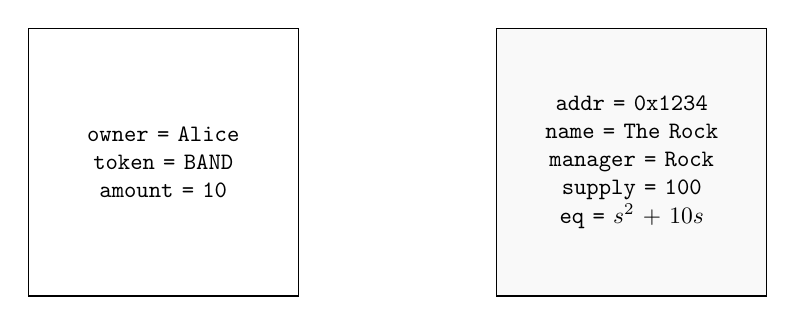
\begin{tikzpicture}[node distance=7cm]
\node (node1) [utxo] {
    owner = Alice \\
    token = BAND \\
    amount = 10
};

\node (node2) [contract,right of=node1] {
    addr = 0x1234 \\
    name = The Rock \\
    manager = Rock \\
    supply = 100 \\
    eq = $s^2 + 10s$
};
\end{tikzpicture}
\caption{Left box is a UTXO representing 10 BAND token owned by Alice. Right box is a contract representing the current state of community token ``The Rock'' living at static address {\tt 0x1234}, with Rock as the community manager, current token supply of 100 The Rock, and value-supply equation of $V(s) = s^2 + 10s$.}
\label{fig:utxo-contract-example}
\end{figure}

\subsection{On-Chain Price Oracle} \label{sec:on-chain-px-oracle}
BAND protocol is built to be aware of external off-chain price information. This allows on-chain fiat pricing in Product Token insurance contracts (\Cref{sec:product-token}), tradable UTXOs (\Cref{sec:marketplace}), and permission contracts (\Cref{sec:permission-contracts}). To achieve this goal, BAND protocol requires that every block must contain the following price information. Note that this list can be extended later as necessary.

\begin{itemize}
\setlength\itemsep{0em}
\item $P_{\mathit{BNDUSD}}$ : The volume-weighted average price of BAND token and US Dollar across all cryptocurrency exchanges.
\item $P_{\mathit{EURUSD}}$ : The conversion rate between Euro and US Dollar.
\item $P_{\mathit{GBPUSD}}$ : The conversion rate between British Pound and US Dollar.
\end{itemize}

For a block with price information to be committed, the majority of consensus participants must agree on the price values (Refer to~\cref{sec:dPOS} for consensus detail). Nodes will accept any price within 1\% error threshold. To prevent one bad price from having a direct influence on the token pricing, the protocol uses the median price among 120 consecutive blocks as one valid price data point. Given block time of one second, a single data point comes from a median price over a period of two minutes. Additionally, to prevent short-term price manipulation, on-chain price is the median among last 30 data points. Thus a price at any point is the median of price in the past one hour. Notice that with this approach, the on-chain price will not change more frequently than every two minutes. This reduces chances of transaction, which derives BAND token price based on $P_{\mathit{BNDUSD}}$, getting invalidated when the blockchain is backlogged and potentially lead to more backlogged transactions.

\begin{figure}[!ht]
 \begin{adjustwidth}{-0.5cm}{}
\begin{tabular}{c|c|c|c|c|c|c|c|c|c|c|c|c|c|c|c}
 & 1 & 2 & 3 & 4 & 5 & 6 & 7 & 8 & 9 & 10& 11& 12& 13& 14& 15\\ \hline
datapoint 1 & {\color{cyan} 32} &7 &66 &{\color{cyan} 42} &55 &67 &61 &41 &38 &1 &{\color{cyan} 27} &59 &33 &45 &21 \\
datapoint 2& 18 &52 &{\color{cyan} 62} &60 &{\color{blue} 37} &64 &75 &65 &{\color{cyan} 35} &34 &5 &3 &15 &14 &56 \\
datapoint 3& 8 &{\color{cyan} 44} &74 &29 &23 &{\color{cyan} 43} &{\color{cyan} 48} &17 &25 &51 &4 &46 &{\color{cyan} 36} &{\color{cyan} 39} &69 \\
datapoint 4& 47 &70 &12 &71 &49 &30 &13 &20 &53 &{\color{cyan} 9} &73 &{\color{cyan} 26} &54 &63 &72 \\
datapoint 5& 40 &31 &58 &19 &16 &10 &28 &{\color{cyan} 24} &22 &2 &57 &11 &50 &6 &{\color{cyan} 68} \\
\end{tabular}
\caption{Illustration of median of medians algorithm over 75 data points split into 15 groups of 5. Cyan numbers are the medians of their groups. The median of medians is shown in blue. In BAND protocol, price information for each group is collected every second over the period of 2 minutes (group size of 120). The on-chain price is the median over the most recent 30 groups.}
\end{adjustwidth}
\end{figure}

\subsection{BAND Token}
BAND token is the primary network token native to BAND Protocol. At blockchain level, an amount of BAND tokens is represented as a UTXO containing the amount and its owner's address. BAND token serves three primary functionalities.
\begin{enumerate}
\setlength\itemsep{0em}
\item Secure the network and prevent network spam through staking.
\item Act as network token to provide global liquidity to each of the Community Tokens through continuous bonding curve model.
\item Serve as a future governance token to vote on protocol upgrade as well as curating a list of future communities.
\end{enumerate}

\subsubsection{Staking}
The protocol allows network participants to stake their BAND tokens in exchange for consensus voting power (See~\cref{sec:dPOS}) and network bandwidth (See~\cref{sec:incentives-and-fees}). To stake BAND token, the owner of a BAND UTXO sends a {\tt STAKE} transaction to the network transforming the BAND UTXO into a staked BAND UTXO of the same amount. To un-stake the token, the owner sends an {\tt UNSTAKE} transaction, effective undoing the previous {\tt STAKE} transaction. Staked BAND UTXOs are different from UTXO because they cannot be spent until they get transformed back to BAND UTXOs.

\begin{figure}[!h]
\centering
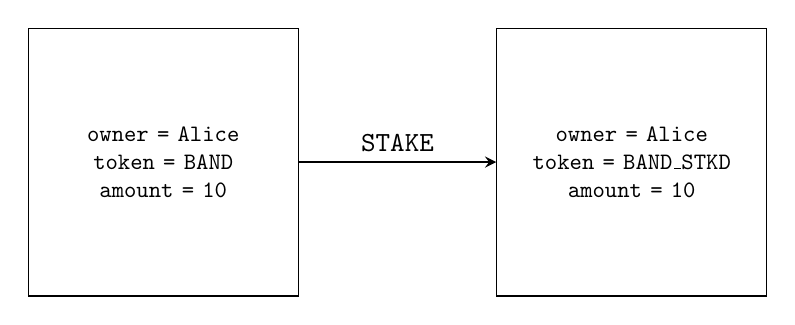
\begin{tikzpicture}[node distance=7cm]
\node (node1) [utxo] {
    owner = Alice \\
    token = BAND \\
    amount = 10
};

\node (node2) [utxo, right of=node1] {
    owner = Alice \\
    token = BAND\_STKD \\
    amount = 10
};

\draw [arrow] (node1) -- node[anchor=south] {{\tt STAKE}} (node2);
\end{tikzpicture}
\caption{An action of staking 10 BAND token by Alice}
\label{fig:utxo-stake}
\end{figure}

\subsubsection{Bonding}
BAND tokens are used as collateral to issue any Community Token through a continuous bonding curve. After Community Manager defines a bonding curve equation, anyone can buy Community Token by sending BAND token to the contract. Conversely, anyone can sell Community Token back to the contract to receive BAND Token. The buying and selling prices are algorithmically adjusted based on the Community Token's circulating supply and the bonding curve equation. Please refer to~\cref{sec:community-token} for more technical discussion regarding Community Token.

Similar to how there is a long tail of {\tt ERC20 Token}, there will be a long tail of less liquid Community Token as communities are fragmented. BAND token acts as a network token to provide global liquidity between all Community Token and thus anyone can buy, sell or switch between any Community Token with instant liquidity.

% As many communities develop on Band Protocol, there will be many specific community tokens being issued. While there will be major communities where there are many transactions to buy and sell Community Token, there will also be a long tail of community tokens with less liquidity as communities are fragmented. By bonding their community tokens to Band Token, Band Token acts as a network token that ensures instant liquidity between all community tokens.

\subsubsection{Governance and Token-Curated Registries}
Once BAND protocol is deployed and used by multiple communities, its internal logic cannot be changed easily. To upgrade, one must deploy new contract that may potentially fork the community and cause disruption among existing, working communities. Upgrade can affect security and usability of the system and therefore cannot be taken lightly. BAND Token will act as a governance token for stakeholders in every community to vote for future decentralized upgrade and governance issues. This ensures that every stakeholders will thoroughly vet new protocol upgrades and vote in favor of those that truly align with the best interest of the communities.

While initially the first set of communities will be strictly handpicked, as project moves toward complete decentralization, there will be a mechanism to maintain a registry of communities and associated Community Manager who has the right to create and maintain the community. Since there can potentially be bad actors who impersonate others, there need to be a trusted source of registry that maintains ownership right. Hence this requires a token-curated registry where BAND Token stakeholders will verify and vote to approve community creation. In order to create a community, Community Manager must submit their application along with BAND Token as a collateral, and BAND Token stakeholders must either accept or reject such application. Since the value of BAND Token tie closely to the quality of communities being developed on the protocol, stakeholders have strong incentive to maintain a high quality list of communities.

\newpage
\section{BAND Protocol}

\subsection{Community Token}

\subsubsection{Value-Supply Equation}

\subsubsection{Maximum Supply}

\subsubsection{Price Spread}

\subsubsection{Purchase Flow}

\subsection{Product Token}

\subsubsection{Issuance}

\subsubsection{Redemption}

\subsubsection{Beneficiary}

\subsection{Marketplace}

\subsection{Subscription Model}

\subsubsection{Staking Contract}

\subsubsection{Discount Token}

\subsection{Attention Contracts}

\subsection{Service API Contracts}

\section{Client Layer}

\subsection{Campbase}

\subsection{Problem Definition}

\subsection{Solution}

\subsubsection{Story Feed}

\subsubsection{Fan Feed}

\subsubsection{Event}

\subsubsection{Subscription}

\subsubsection{Store}

\subsection{Community Manager}

\subsection{Consumers}

\section{Roadmap}

\bibliographystyle{unsrt}
\bibliography{paper}

\end{document}
